\chapter{3D CNN approach}
\section{Introduction}
\begin{figure}[h]
    \centering
    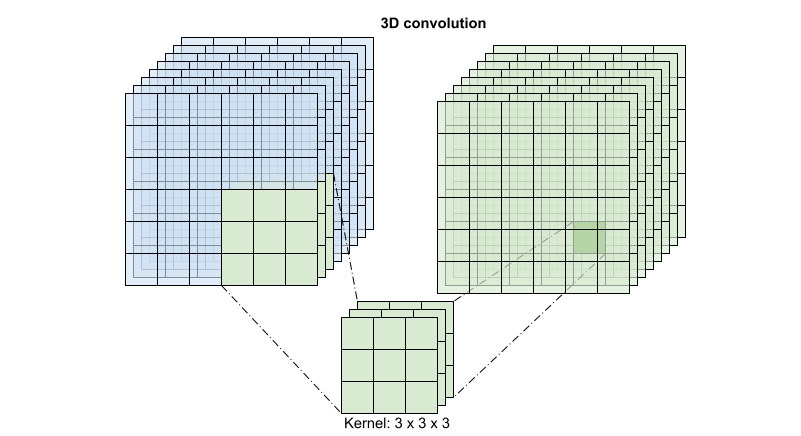
\includegraphics[width=\textwidth]{./images/3DCNN.png}
    \caption{How a 3D CNN works}
    \label{fig:How3DCNNWorks}
\end{figure}

2D CNN networks operate by applying convolutions spatially, traversing both the horizontal and vertical dimensions of the input data. The convolutional operation employs 2D kernels, usually specified in terms of height and width. Channels, representing different aspects of the input data (e.g., Red, Green, Blue in color images), are a common feature of 2D CNNs.

On the other hand, 3D CNNs extend the convolutional approach to three-dimensional data, a structure commonly found in video or volumetric datasets. The input to a 3D CNN includes not only width and height but also a third dimension, often representing depth or frames in the temporal domain. Consequently, the kernels used in 3D CNNs are three-dimensional, incorporating depth, height, and width. This extension allows the model to capture spatial features across multiple frames, introducing a temporal aspect to the convolutional operation. In addition to the spatial channels, 3D CNNs often have an extra channel to account for the temporal dimension, making them particularly suitable for tasks involving video analysis and scenarios where temporal information is crucial like our \textit{violence recognition} problem.

While 2D CNNs have proven effective for traditional image-related tasks like classification, object detection, and segmentation, 3D CNNs are specifically designed for applications where volumetric or temporal information is essential. However, the use of 3D CNNs comes at a higher computational cost due to the increased complexity introduced by the additional dimension. This would proved to be a problem for us due to the fact that we did not have a GPU at our disposal and the one provided by Google Colab were not capable enough to handle big models and big data-sets.

\section{Implementation}
As explained in the "Frame extraction" section, the pickles approach allowed us to generate files containing the data needed to train and test the model. The \textit{number of frames} and the \textit{fps} values for each pkl\_config were used to test the same model on different input data like burst of 1, 2 or 3 seconds. As shown in Fig. \ref{fig:3DCNNschema}, the model is a very simple one, with 2 convolutional layers, 2 max pooling layers and 1 fully connected. The idea is not to dwell on the model and how improve it, but to show that the addition of "context" to the input data, in this case the temporal dimension, allows the model to achieve better results independently form the complexity of the model.
\begin{figure}[]
    \centering
    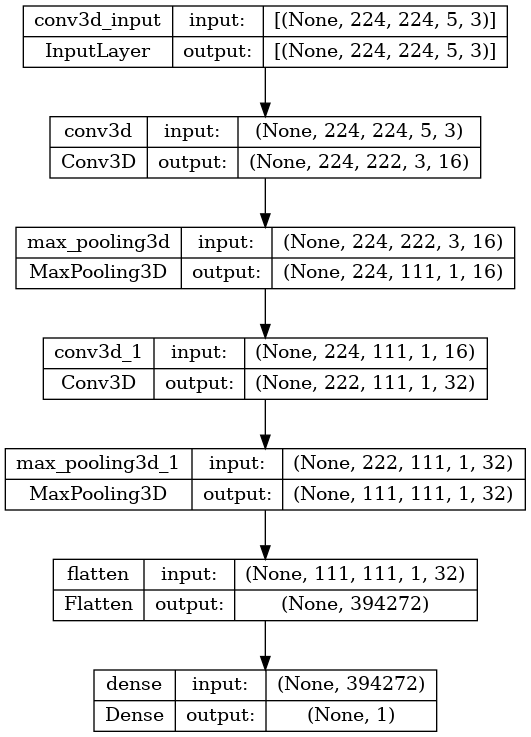
\includegraphics[width=0.8\textwidth, height=0.6\textwidth, keepaspectratio]{images/3D9CNNschema.png}
    \caption{Schema of the 3D CNN}
    \label{fig:3DCNNschema}
\end{figure}

The very first test was done with number of frames (NoF) equal to 5 and fps equal to 5, meaning that the model would received burst of 1 second each. Fig. \ref{fig:First3DCNNconfusionMatrix} shows an interesting result, it is very similar to the best 2D scratch one but it has slightly better recall score in general, but loses al lot regarding the violence recall.

\begin{figure}[]
    \centering
    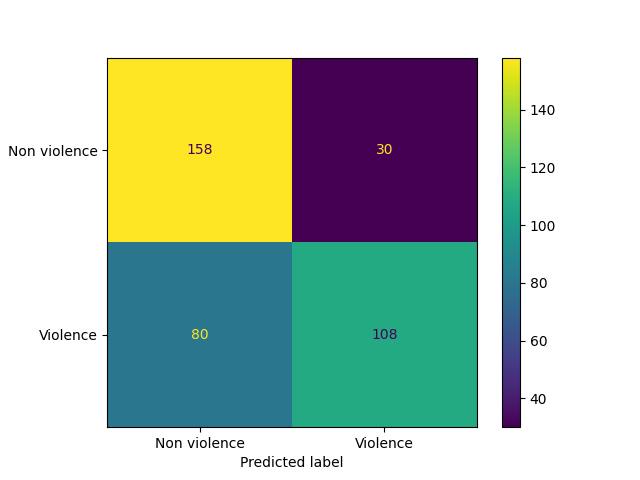
\includegraphics[width=0.8\textwidth]{images/7f2d-testGiacomo3D9-9fcf-conf_matrix.png}
    \caption{Confusion matrix of the first 3D model}
    \label{fig:First3DCNNconfusionMatrix}
\end{figure}

The second test was done with NoF equal to 10 and fps equal to 5, meaning that the model would received burst of 2 seconds each. This was done to see if the model would improve with more context, since 1 second of video is not a lot especially for the longer ones. 

\begin{figure}[]
    \centering
    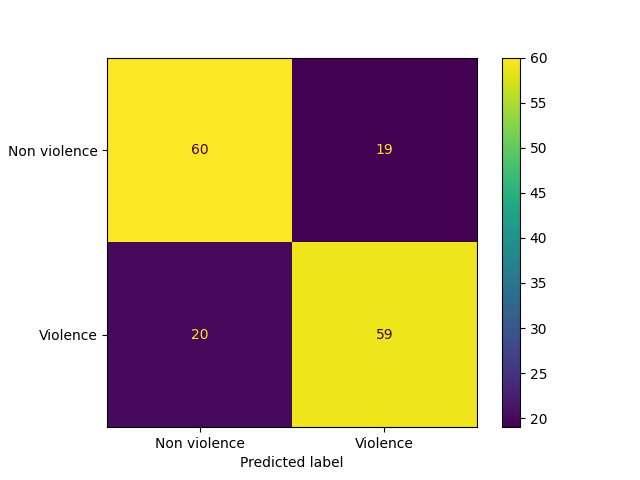
\includegraphics[width=0.8\textwidth]{images/ce07-testGiacomo3D3-9fcf-conf_matrix.png}
    \caption{Confusion matrix of the second 3D model}
    \label{fig:Second3DCNNconfusionMatrix}
\end{figure}

Finally the third test was done with NoF equal to 15 and fps equal to 5, meaning that the model would received burst of 3 seconds each. Keep in mind, however, that since some of the original dataset is made of videos shorter than 3 seconds both training and test set are reduced. This means that the result are to be taken lightly since they are not representative of the whole dataset. In addition the previous model needed to be made lighter to avoid making it to complex for the smaller dataset, the new schema can be seen in Fig. \ref{fig:3D3CNNschema}. The result show in Fig. \ref{fig:Third3DCNNconfusionMatrix} is the best one so far, with a very good recall score for both the classes. This is due to the fact that the model has more context to work with and can better understand the situation.

\begin{figure}[]
    \centering
    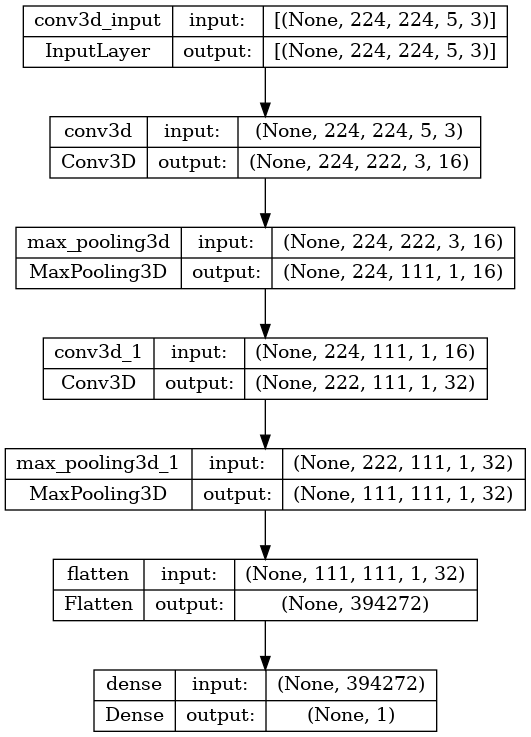
\includegraphics[width=0.8\textwidth, height=0.6\textwidth, keepaspectratio]{images/3D9CNNschema.png}
    \caption{Schema of the "simpler" 3D CNN}
    \label{fig:3D3CNNschema}
\end{figure}


\begin{figure}[]
    \centering
    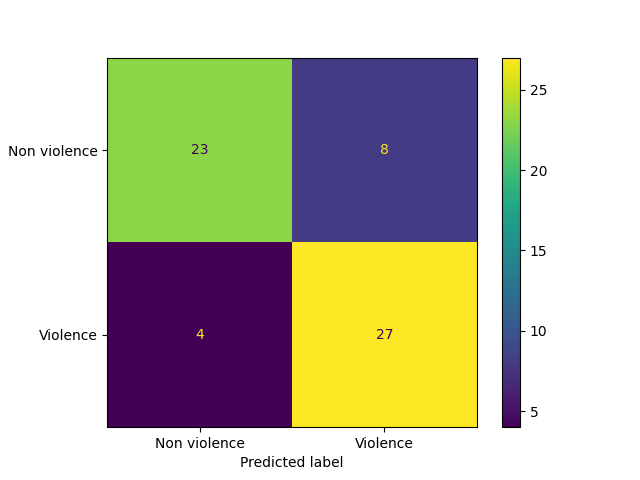
\includegraphics[width=0.8\textwidth]{images/71d5-testGiacomo3D3-9fcf-conf_matrix.png}
    \caption{Confusion matrix of the third 3D model}
    \label{fig:Third3DCNNconfusionMatrix}
\end{figure}



\chapter{Conclusion}
Finally a table with the accuracy of all the models can be seen in Tab. \ref{tab:3DCNNtable}. This proves that the 3D CNN approach is a valid one and that it can be used as an alternative to the 2D CNN one. However, the 3D CNN approach is more computationally expensive and requires more time to train and test, but it can achieve better results. Another thing to keep in mind is that the 3D CNN approach seems to gain from longer burst of video, giving the model more "context". This means that the 3D CNN approach is more suitable for real time analysis of CCTV footage, where the model receive burst of videos and is able to decide if there is violence or not by analyzing the evolution of the features over time. This is not the case for the 2D CNN approach that is more suitable for static images, where the model is able to decide if there is violence or not by analyzing the features of a single frame, but it is not able to understand the evolution of the situation over time.

\begin{table}[h]
    \centering
    \resizebox{\textwidth}{!}{%
    \begin{tabular}{c|c|c|c|}
    \cline{2-4}
                                                             & \textbf{Accuracy} & \textbf{Violence recall} & \textbf{Non violence recall} \\ \hline
    \multicolumn{1}{|c|}{\textbf{Best 2D scratch}}           & 0,7048            & 0,9095                   & 0,5                          \\ \hline
    \multicolumn{1}{|c|}{\textbf{Best Resnet}}               & 0,7643            & 0,6952                   & 0,8333                       \\ \hline
    \multicolumn{1}{|c|}{\textbf{Best accuracy efficienNet}} & 0,7762            & 0,7191                   & 0,8333                       \\ \hline
    \multicolumn{1}{|c|}{\textbf{Best recall efficienNet}} & 0,7571            & 0,8857                   & 0,6285                       \\ \hline
    \multicolumn{1}{|c|}{\textbf{First 3D model}}            & 0,7074            & 0,5744                   & 0,8404                       \\ \hline
    \multicolumn{1}{|c|}{\textbf{Second 3D model}}           & 0,7532            & 0,7468                   & 0,7595                       \\ \hline
    \multicolumn{1}{|c|}{\textbf{Third 3D model}}            & 0,8065            & 0,8710                   & 0,7419                       \\ \hline
    \end{tabular}%
    }
    \caption{Models accuracy}
    \label{tab:3DCNNtable}
\end{table}
